
\section{Interference management}

The interference management component of \cf needs to solve a distributed channel allocation problem, 
and in particular it needs to determine: {\em (1) What share of resource blocks should each network get?} and 
{\em (2) Which particular resource blocks should each access point use and how should it adjust it dynamically?}

Similar allocation problems have been well studied in other contexts, for example in \wf or LTE SON. 
However, there are several specifics that make this problem in the \cf context unique. 
Firstly, \cf is required to manage interference without explicit coordination, unlike conventional LTE networks (c.f.~\cite{smallcellbook, fermi}). 
Secondly, an LTE access point can transmit on several resource blocks at once, 
and it can change the schedule in each subframe (1ms interval) without any overhead. 
Further, an LTE client can always sense the status of all resource blocks, even the ones it is not receiving in. 
This is very different from \wf where a node can only use and sense one channel at a time, and has significant overhead when changing channels. 
Thirdly, if two access points transmit on the same resource block and these transmission interfere at a client, the client will not receive its transmission. This is in contrast with \wf where nodes use CSMA to further avoid interference among nodes that share the same channel. 
Thus, in comparison with \wf, \cf has better sensing and frequency scheduling mechanisms, but the consequences of wrong decisions are more detrimental. 

Next, we discuss \cf's distributed interference management algorithm. 
\cf schedules resources in terms of subchannels, where a subchannel is defined to be the minimal set of resource blocks that can be scheduled in LTE and for which we can get channel quality information (Section~\ref{sec:sensing}). 
In practice, there are 13 such subchannels on 5MHz channel and 25 subchannels on a 20 MHz channel. 
The following discussion focuses on the downlink because the uplink is much less saturated; 
yet, the uplink can be managed similarly.

We start by describing the sensing mechanisms \cf uses to learn about its neighborhood and then we discuss the distributed share calculation and the distributed subchannel selection phases. %, described previously in Section~\ref{sec:archint}.
We then present the discussion about the convergence properties of the algorithm as well as its theoretical guarantees, showing that 
the algorithm is guaranteed to converge to the pre-calculated share allocation in $\log{(\mbox{\# users})}$ steps. 



\subsection{Sensing mechanisms}
\label{sec:sensing}

Like WiFi, the \cf interference mitigation algorithm relies on sensing information from the environment. The \cf access point leverages standard LTE radio primitives to estimate the following:

\noindent{\bf Number of active clients.} In LTE, each client sets up a connection by sending PRACH preambles. 
This is a special preamble that is used by access points to identify a new node and assign spectral resources to it. 
In \cf, we extend this mechanism, and each access point is equipped with an additional PRACH detector that can sense PRACH preambles from \emph{clients it is not serving} (Section~\ref{sec:pracheval}).
This is used to estimate the number of active clients. \todo{Note that adding additional PRACH detector does not require any invasive change to LTE infrastructure \ref{}}
The transmit power difference between a client and \eNB is up to 10dB, 
and a PRACH detector can reliably detect preambles at -10dB SNR~\cite{prach}. 
Thus, any client whose PRACH is detected is likely to be affected by transmissions from the \eNB. 
\cf nodes use PDCCH-order RACH primitive of LTE to solicit PRACH preambles every second~\cite{36_213}. 
This allows sensing nodes to expire each estimate after 1 second and account for nodes that become inactive. 


\noindent{\bf Client interference in each subchannel.} When instructed by its access point, LTE clients report 
back a channel quality indicator (CQI). 
The \cf access point configures its clients to send higher layer-configured aperiodic mode 3-0, sub-band CQI reports~\cite{36_213} every 2 msec. 
It tracks the maximum reported CQI for each client and \emph{each subchannel} over a period of time. 
Drops in CQI values indicate interference with a client in that subchannel (Section~\ref{sec:eval_cqi}). 


\subsection{Distributed Share Calculation}
\label{sec:share-calculation}

%Every \eNB is set to detect PRACH preambles from any user but responds with a RAR message only to its own users.
%The \eNB keeps track of the number of the unique PRACH preambles it has received in the previous round.

%In our implementation, each \eNB $i$ computes its share for all its users using the following procedure. (See %Figure~\ref{fig:dsc} for pseudo-code.) 


Consider \eNB $i$. Let $\mathcal{S}$ be the total number of subchannels available, 
$\id{NP}_i$ the number of estimated active clients and 
$\id{N}_i$ the number of active clients associated with \eNB $i$. 
We estimate $\id{NP}_i$ using the PRACH detector.


First, for each active client, the \eNB $i$ reserves 
%$$\frac{\mathcal{S}}{\id{NP}_i}$$ 
$\mathcal{S} / \id{NP}_i$ 
distinct shares, giving it a total share of 
%$$\id{S}_i =  \id{N}_i * \frac{\mathcal{S}}{\id{NP}_i}$$ 
$\id{S}_i =  \id{N}_i * \mathcal{S} / \id{NP}_i.$ 
This is how we ensure \emph{frequency fair-sharing.} All $\id{NP}_i$ clients that \eNB $i$ interferes with should get enough non-interfering subchannels. 

Because of imperfect sensing, this approach can occasionally underestimate the target shares and reduce efficiency, but it is still more efficient than Wi-Fi or LTE, as our evaluation in Section~\ref{sec:eval} shows. An \eNB can also initially overestimate the share available to some of the clients, in which case the scheduler will later automatically assign these to its other clients. This is further discussed later in \ref{sec:asymmetry}.
\todo{copy the discussion from the appendix to correct location.} 

%one of its client but if the client does not actually have enough interference free subchannels, 
%the scheduler will make sure that the additional subchannels are either used for some other client of the same \eNB or are left free.


%Further, if an \eNB initially overestimates its share because of imperfect sensing, it will use the $\id{free}_{i, j}$ estimator to back off from its initial demand, allowing other nodes  to achieve their share (discussed in Section~\ref{sec:asymmetry}).

%The unused total share of the \eNB is then divided among users which observe more free channels than their current share. 
%The total demand of the \eNB will then be 
%$$\sum_{user\, j} \id{share}_{j}.$$ 

%We note that a client may not get any share as an outcome of this procedure. 
%However, this does not mean that it will starve. As described next, our scheduler will still try to schedule all clients; 
%however, clients that got no share are more likely to get starved because of excessive interference. 



%% \centering
%% \begin{minipage}{.45\textwidth}
%%   \centering
%% \begin{algorithmic}[1]
%%  {\small
%% %  \CommentLine{Lease the line corresponding to \texttt{addr} for \texttt{len} cycles}
%% \Function{ShareCalculation}{ \eNB $i$ } 
%% 	\For{ each user $j$ }
%% 		\State $\triangleright$ Reserve subchannels per user 
%% 		\State $\id{share}_j  \gets \min( \lfloor \mathcal{S} / \id{NP}_i \rfloor, \id{free}_{i, j} )$ 
%% 	\EndFor
%% 	\State $\triangleright$ Compute unused subchannels
%% 	\State $\id{extra}_i \gets ( \sum_{ j} \id{free}_{i, j} - \sum_{j} \id{share}_j) $ 
%% 	\State $\triangleright$ Users with underutilized subchannels
%% 	\State $\id{cand}_i \gets$ users with $(\id{free}_{i, j} > \id{share}_j)$ 
%% 	\If { $\id{extra}_i$ > 0 }
%% 		\State allocate $\id{extra}_i$  to users in $\id{cand}_i$	
%% 	\EndIf
%% 	\State \textbf{return} $\sum_{\id{user} j} \id{share}_j $
%% \EndFunction
%% }
%% %\Statex
%% \end{algorithmic}
%% %\end{algorithm*}
%% \vspace{-6pt}
%% \caption{{Distributed share calculation.}}
%% \vspace{-12pt}
%% \label{fig:dsc}
%% \end{minipage}\hspace{3em}



\begin{figure}[tbp]
\begin{minipage}{.45\textwidth}
\begin{algorithmic}[1]
 {\small
%  \CommentLine{Lease the line corresponding to \texttt{addr} for \texttt{len} cycles}
\Function{Hopping}{ \eNB $i$ } 
	
	%\State $\triangleright$ Initialization:

	%\For{ each user $j$ }
		
		\State $C_j \gets \id{S}_i$ subchannels, picked randomly
		\For{ each subchannel $k$ }
				\State $\triangleright$ Draw exponential bucket value 
				\State $b_k^i \gets \texttt{exp}(\lambda)$ 
		\EndFor
	%\EndFor
	
	\For{ each phase }
		\For{ each occupied subchannel $k$ }
			\If{ $b_k^i = 0$ }
				\State $k' \gets$ subchannel with maximum utility
				\State swap $k$ with $k'$ 
			\EndIf
		\EndFor
	\EndFor
\EndFunction
}
%\Statex
\end{algorithmic}
\vspace{-6pt}
\caption{{Hopping Procedure.}} 
\vspace{-12pt}
\label{fig:hopping}
\end{minipage}
\end{figure}


 
%$$Share_i = \frac{NA_i}{ NR_i} \times Number of SubChannels$$ 
%where $NA_i$ is the number of active users associated with $eNB_i$ and $NR_i$ is the number of unique RACH preambles received by $eNB_i$ in the previous round. The $NR_i$ approximates the number of clients that can hear $eNB_i$ and will hence be affected by $eNB_i$ transmissions. 
%$eNB_i$ then distributes $Share_i$ equally among its active users, i.e every user gets $\frac{Share_i}{NA_i}$.
%If for a user $j$, $\frac{Share_i}{N_i} > Free_{ij}$, $j'$s share is reduced to $Share_{ij} = Free_{ij}$, and the remaining share $(\frac{Share_i}{N_i} - Free_{ij})$, is distributed among users who can take more share i.e. users for which $(\frac{Share_i}{N_i} < Free_{ik})$. If no user is available to take up the remaining share $eNB_i$ reduces its share to $$Share_i = \sum_{j=1}^{NA_i} Share_{ij}$$


\subsection{Distributed Subchannel Selection}
  \label{sec:channel-selection}
  
We now describe the process by which an \eNB selects and schedules subchannels. 
For clarity, we split this  into the following procedures. 
  
%An \eNB $i$ assigns subchannels to its clients as follows (see Figure~\ref{fig:hopping} for pseudocode).

%  \label{hopping}
\noindent{\bf Subchannel Hopping.} 
Initially, \eNB $i$ randomly picks $\id{S}_i$ subchannels. 
For each subchannel $k$ chosen by $i$, a random bucket value $b^{i}_{k}$ is drawn from an exponential distribution with mean $\lambda$ (we found $\lambda = 10$ to be a good choice experimentally). 
Clients associated with an \eNB send periodic subchannel CQI reports. 
In all subsequent phases, if a subchannel bucket value $b^{i}_{k}$ reaches $0$, the \eNB $i$ gives up subchannel $k$, and chooses a new subchannel based on a function of CQI values reported by the users that were scheduled on subchannel k.
Our implementation chooses the new subchannel that has maximum utility, where utility is defined as the sum of throughput achieveable (as estimated from the CQI reading) by all the clients scheduled over the previous subchannel in the recent past scaled by the fraction of time that client was scheduled. 
See Figure~\ref{fig:hopping} for pseudocode. 

%  \label{bucket-update}
\noindent{\bf Bucket Updates.}
    Each \eNB updates its bucket values corresponding to employed subchannels periodically as follows. For every client $u_j$ scheduled on the subchannel during the previous period

%\begin{itemize}
%\item 
\vskip 2pt
\noindent $\bullet$ If client $u_j$ observes subchannel $k$ as \emph{good} (according to the last CQI report), then $b^{i}_{k}$ stays unchanged.
%\item 
\vskip 2pt
\noindent $\bullet$ Otherwise we interpret subchannel $k$ as being a \emph{bad} for \eNB $i$. Consequently, the bucket value $b^{i}_{k}$ is decremented to $b_k(t+1) = b_k(t) - frac_j$, where $frac_j$ is the fraction of time that $u_j$ got scheduled on subchannel $k$ during the last period.
\vskip 2pt
%\end{itemize}
\todo{The random bucket values and bucket update procedure would ensure that two interfering users scheduled on a subchannel would not give up the subchannel at the same time hence ensuring both users get non-interfering subchannels eventually. }
The subchannel hopping and bucket update procedures are similar to other Markovian schemes (e.g. IQ-hopping~\cite{iqhop} and references therein) but are adapted to address the main differences between LTE and Wi-Fi, discussed at the beginning of this section.

%% In particular, while WiFi has a well defined channel and each WiFi node only
%% needs to select one channel to hop, in \cf, we have fine-grained sharing using OFDMA, where a frame may contain data to
%% different clients in different subchannels over time. 
%% Moreover, we can no longer rely on frame-level ACKs used in IQ-hopping to
%% determine how long to stay on a subchannel, so we rely on CQI measurements which is reported per subchannel.


%% \noindent {\bf Scheduling.} Whole resources are allocated to an access point using the procedures above, 
%% they are not strictly assigned to any specific client. The interference created by an access point does not depend on which clients are scheduled in which subchannels, 
%% but only on which subchannels are overall used by the access point. Thus, the access point has a flexibility to modify the scheduler without affecting the rest of the network. 
%% This allows us to ensure that resource reservation is decoupled from resource scheduling for clients. 

%% Once the \eNB attains its subchannel demand, it schedules its users in its reserved subchannels according to a \emph{proportional fair schedule}\cite{propfair}. 
%% The main reason for this is to improve efficiency; If all flows are fully saturated, the proportional scheduler will tend to schedule traffic 
%% according to the way resources are allocated. However, if one of the clients is idle, the access point will assign the corresponding resource to other clients in order to maximize spectral efficiency 
%% and provide work conservation.  


\noindent {\bf Channel re-use.} Clients very close to their respective access points are not likely to interfere with anyone else;  
hence, it would be beneficial to schedule them in the same subchannels across different networks to maximize throughput. 
%otherwise some of the access points might not be able to get interference free channels even when the neighbouring access points only transmit on their conservative share of subchannels.
% (see figure~\ref{fig:asym}(a) for an example). 
This is difficult to accomplish without coordination across networks and access points.
To achieve this, we use the following heuristic.
%Each client maintains a leaky bucket corresponding to each channel it is assigned to. 
%The client will move to a channel \emph{of lower index} if this channel is detected as \emph{free} for a certain contiguous period of time. 
The access point will give up subchannel $i$ and move to a subchannel \emph{of lower index} if this subchannel is detected as \emph{free} for a certain contiguous period of time, by all of the users that were scheduled on the subchannel $i$ in the recent past. 
The idea is that clients which experience low interference (such as the ones close to access points), 
will gradually move towards lower-index subchannels, spontaneously self-organizing. 
Channel re-use allows for fast convergence and upto 2x gain in throughput for exposed clients as seen in our experiments. 

%the network efficiency is significantly improved 
%{\bf XXXX ADD Some number on how much channel re-use improves results XXX}

%We defer theoretical analysis and discussion of the algorithm to the appendix.


\begin{figure}[htb!]
  %\hfill
  %\begin{minipage}{0.33\textwidth}
  %  \centering
  %  (a)
  %  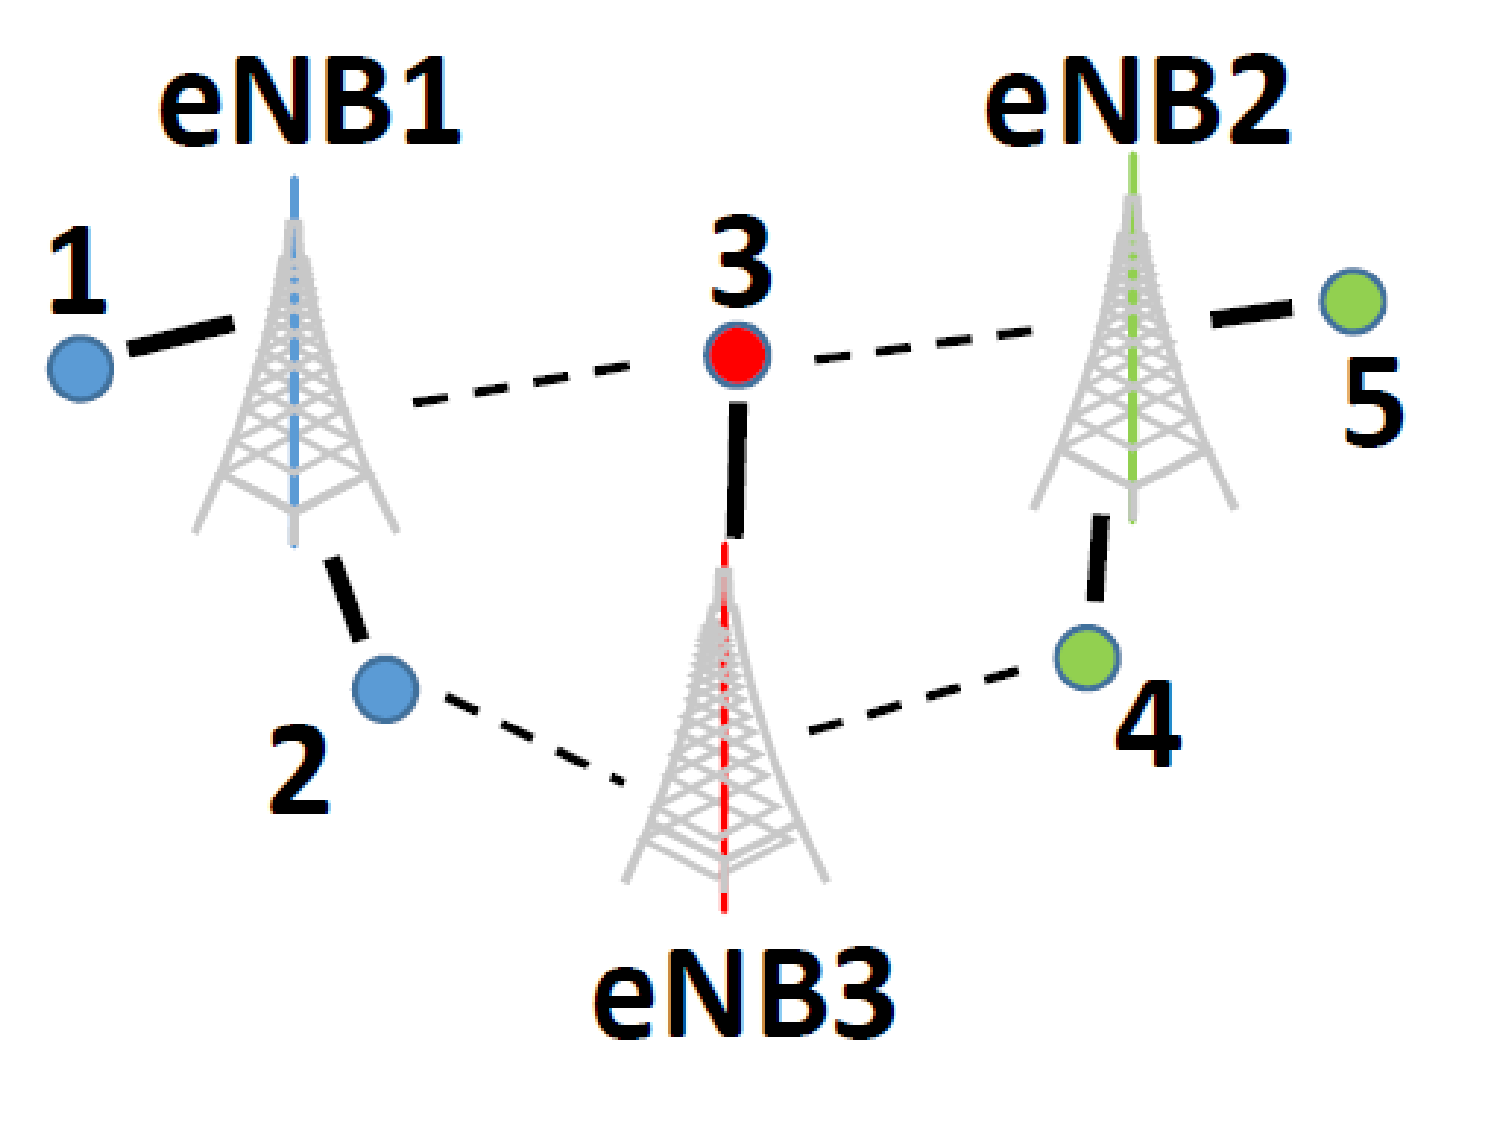
\includegraphics[width=\textwidth,height=0.6\columnwidth]{./figs/pack.pdf}
  %\end{minipage}
  %\hspace{1pt}
  \begin{minipage}{0.23\textwidth}
    \centering
    (a)
    \vfill
    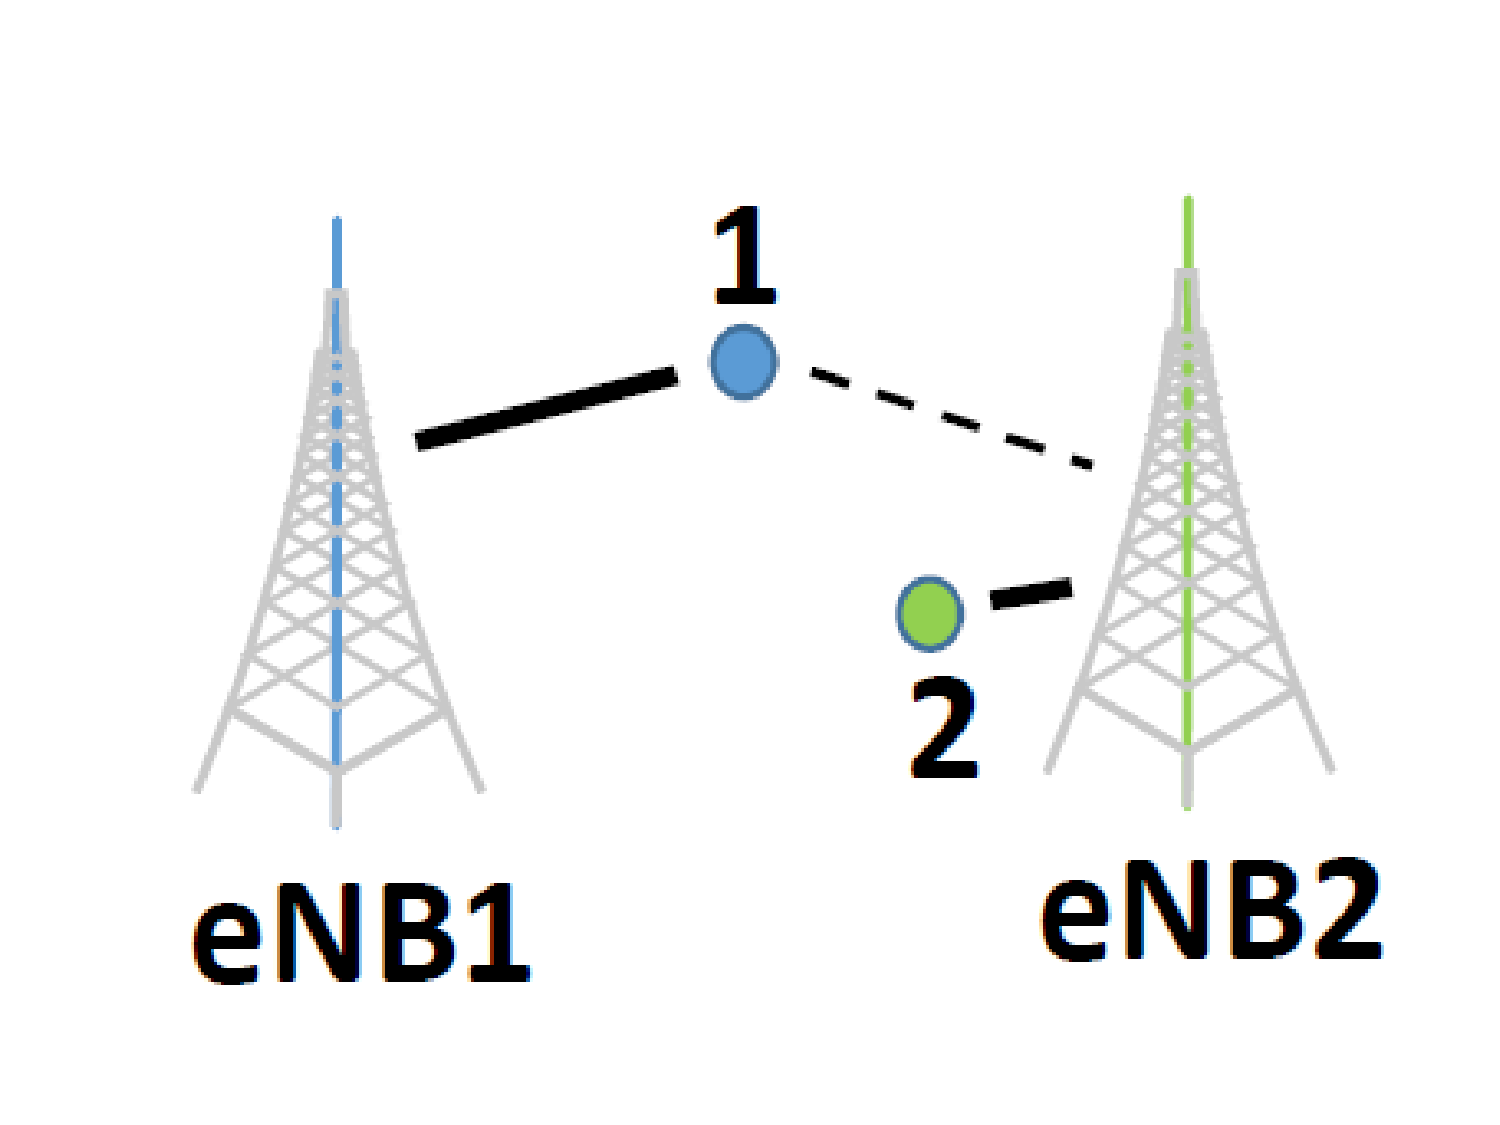
\includegraphics[width=\textwidth,height=0.6\columnwidth]{./figs/over.pdf}
  \end{minipage}
  \begin{minipage}{0.23\textwidth}
    \centering
    (b)
    \vfill
  \includegraphics[width=\textwidth,height=0.6\columnwidth]{./figs/under.pdf}
  \end{minipage}
  \hfill
  \caption{Lines reflect associated clients to access points while dashed lines reflect interference. }
%(a) Importance of channel re-use. client 3 can only get its share if access points 1-2 schedule their clients on same two channels. 
%(a) Information asymmetry with two total channels. access point 1 overestimates his share because it cannot sense client 2. (b) Informatrion assymetry with 4 total channels. 
%access point 2 has a share of 1, and while access point 1 can increase his share to 3, 
%it only reserves his fair-share, i.e., 2 channels because it does know how many subchannels 2 is using (1 due to clients 3-5)}
  \label{fig:asym}
\end{figure}


\subsection{Effects of information asymmetry}
\label{sec:asymmetry}


Wireless sensing depends on node location, and different nodes will obtain different views of the network. 
Every distributed wireless coordination protocol has to deal with this information asymmetry. 
The best known examples of information asymmetries in WiFi are exposed and hidden terminals. 
The distributed share calculation algorithm of \cf also suffers from two cases of information asymmetry, 
described below. 





%\begin{figure*}[t]
% \centering
%    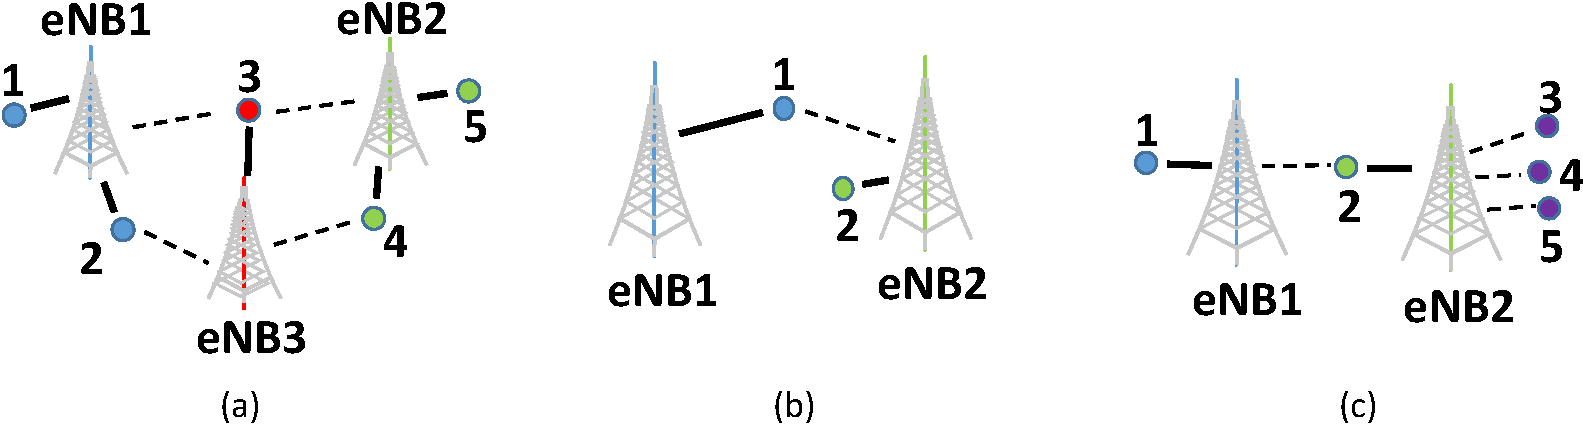
\includegraphics[width=0.9\textwidth, height=0.4\columnwidth]{figs/exampleFigs-crop}
% \caption{Lines reflect associated clients to access points while dashed lines reflect interference. 
%(a) Importance of channel re-use. client 3 can only get its share if access points 1-2 schedule their clients on same two channels. 
%(b) Information asymmetry with two total channels. access point 1 overestimates his share because it cannot sense client 2. (c) Informatrion assymetry with 4 total channels. 
%access point 2 has a share of 1, and while access point 1 can increase his share to 3, 
%it only reserves his fair-share, i.e., 2 channels because it does know how many subchannels 2 is using (1 due to clients 3-5)}
%  \label{fig:asym}
%\end{figure*}




\noindent {\bf Incorrect share:} Figure~\ref{fig:asym}(a) shows an example of incorrect share calculation caused by asymmetric views. 
access point 1 can hear only the PRACH preamble from client 1, whereas eNB2 hears it from both clients 1 and 2. The optimal share for both eNBs is half of the spectrum. 
Because of asymmetry, access point 1 is overestimating its share to be the whole spectrum.

%BR: This is not true. If we don't adjust the share, it will make eNB1 to hop a lot, causing disturbances in the rest of the network...
%This case of information asymmetry is not detrimental to the control plane. It does not affect client 2 because if it did eNB1 would hear it RACH and account for it in the channel allocation. It only affect client1. eNB1 detects this from CQI reports from client1 and adjusts the allocation accordingly and entirely locally. 

This case of information asymmetry is dealt with by the scheduler, \eNB $1$ will sense that there are less free subchannels available than it expected, and will not schedule any transmission in subchannels the client is facing interference on, reducing its effective share. The resulting effective share will still be feasible, allowing the distributed hopping algorithm to converge. However, this share adjustment may not be detected by other neighbors of \eNB $1$, leading to possible inefficiencies.
%in the share calculation algorithm (Figure~\ref{fig:dsc}) 
%through the $\id{free}_{i, j}$ variable. \eNB $1$ will sense that there are less free channels available than it expected, and will update its share. The resulting share will still be feasible, allowing the distributed hopping algorithm to converge. However, this share adjustment may not be detected by other neighbors of \eNB $1$, leading to possible inefficiencies. 

%\begin{figure}[th!]
%  \centering
%    \includegraphics[width=0.45\textwidth]{under}
% \caption{Suboptimal share calculation due to view asymmetry.}
%  \label{underestimation}
%\end{figure}

\noindent {\bf Suboptimal share:} Figure~\ref{fig:asym}(b) shows an example with a total of 4 subchannels, where access point 1 can get one more subchannel since access point 2 can only use one subchannel for its client;
this is because it is interfering with three other clients. Access point 1 limits itself to its estimated share of two subchannels, resulting in under allocation of resources. 
This case of information asymmetry is fundamental of our setup as \eNB $1$ cannot learn about other clients purely from sensing. It can also not be more aggressive in this case as it could unfairly take a share 
from node 2, should the three clients on the right be absent. 

The performance effects of information asymmetries of \cf in general topologies are difficult to analyze precisely. 
In Section~\ref{sec:eval},
 we show that in complex topologies, \cf's performance is comparable to state-of-the-art, centralized resource allocation frameworks for cellular networks~\cite{fermi}.



\subsection{Algorithm Properties}
\label{sec:proof}

%\todo{Dan will fill this in.}
%The reason why this work is our high-level design and the distributed share calculation. The distributed share calculation makes sure that the starting allocation is feasible. This allows us to do packing based on free channels. If the initial share wasn't feasible, the algorithm would have issues converging (Dan has a proof for this). This is why the packing idea is fundamentally suitable for our approach.

We now analyze the properties of the assignment framework given in ~\ref{sec:channel-selection}. 
In particular, we will give a sufficient condition under which the basic hopping algorithm 
(without the channel re-use heuristic) is guaranteed to converge, 
and probabilistic convergence bounds in this case. 

More precisely, we abstract the given setting as an undirected graph $G = (V, E)$, where each vertex $v_i \in V$ corresponds to an \eNB $i$. 
Further, two vertices $v_i$ and $v_j$ are connected by an edge if $v_i$ may interfere with one of $v_j$'s clients, or vice-versa. 
Let $N(v_i)$ denote the graph neighborhood of node $v_i$. 
Vertices share a set of $M$ subchannels, and initially each vertex $v_i$ has integer demand $d_i \geq 0$, which corresponds to the sum of user shares computed by the algorithm. 
Our analysis makes the assumption that, in every neighborhood, there exists a constant factor difference between the sum of demands and the total number of  subchannels.

\begin{eqnarray*}
  \textnormal{There exists a constant } 1 / M < \gamma \leq 1, \textnormal{ such that: } \\ \textnormal{ for every node }  v_i, \sum_{\ell \in N(v_i)} d_\ell \leq (1 - \gamma) M.
\end{eqnarray*}

Further, our analysis models subchannel fading by admitting a probability $0 \leq p < 1$ that a subchannel sensed as \emph{free} (and therefore chosen by the hopping procedure) is in fact unusable by the node. 
This failure event is assumed to be independent of the nodes' random hopping choices, and across hopping rounds. 

We focus on \emph{convergence time}, i.e., the time required for the algorithm to reach a configuration in which each node has its subchannel demand fulfilled, and stops hopping. 
We prove the following. 

\begin{thm}
\label{thm:convergence}
	Under the above assumptions, the algorithm is guaranteed to converge with probability $1$. The algorithm will converge in $O( M \log n / ((1 - p) \cdot \gamma) )$ rounds, both in expectation and with high probability.   
\end{thm}
\begin{proof}
	Let us consider the process by which a node $v$ satisfies a unit of its demand. By assumption, the following hold: 1) the node $v$ will not hop on a subchannel currently occupied by another node $v'$ and 2) since a node $v_\ell$ may only occupy $d_\ell$ subchannels in a round, and $\sum_{\ell \in N(v)} d_\ell \leq (1 - \gamma) M$, there exist at least $\gamma M \geq 1$ subchannels which are available at every hopping attempt. Therefore, given a hopping attempt by $v$, there are two conditions under which it does not succeed in acquiring the channel: either another node makes the same choice, or the channel is faded. These events occur independently, and, by assumption, the probability that node $v$ satisfies one unit of demand in a hopping attempt is at least $(1 - p) \gamma$.  
	
	Since round choices and fading are assumed to be independent across rounds, the expected time for the fixed node to satisfy a unit of demand is $ 1 / (\gamma (1 - p))$. By a Chernoff bound, for any constant $k \geq 2$, there exists a constant $c \geq 1$ such that the probability that the node fails to satisfy a unit after $k \log n / (\gamma (1 - p) )$ consecutive hopping attempts is at most $1 / n^c$. 
	By a union bound on the number of nodes, the probability that there exists \emph{some} node which fails after $k \log n / (\gamma (1 - p ))$ consecutive hopping attempts, is at most $1 / n^{c - 1}$. 
	The claim then follows by noticing that a node's demand is of at most $M$ subchannels. 
\end{proof}


It is interesting to consider the effect of channel packing on convergence. 
Technically, a larger channel slack $\gamma$ may be needed if hopping and packing occur concurrently, as packing may increase collisions. 
However, the fact that packing occurs after the node stops hopping ensures that the two procedures are independent to some degree.
The empirical evaluation confirms that convergence still occurs with packing, even for dynamic traffic patterns. 

